\section{Iterative Prompting}
\label{prompting_method}

As we transition from context mining to utilizing the extracted information in LLM prompts, the next challenge is how to feed this information into the model without overwhelming it. While extracting accurate and relevant context is essential, the model's ability to process that information effectively is just as crucial.

% A significant limitation of many LLM-based approaches is context overload, where the model is fed too much information at once, causing it to lose focus on the most pertinent details. This is especially relevant in network configurations, where dependencies and relationships between different configuration lines can be complex and spread throughout the file.




\mypara{Solution:}
To address these issues, \sysname{} implements an iterative, sequential prompting framework that allows the model to request and process relevant context in stages. Instead of overwhelming the model with all available context at once, \sysname{} enables the model to actively request additional information as needed. This approach enhances the model’s ability to maintain focus, coherence, and overall detection accuracy by allowing it to prioritize and process context more effectively, ensuring that only the most pertinent information is presented at each step.

\mysubpara{1. Initial Prompting:} The process begins by feeding the LLM the specific configuration line under review, along with targeted instructions about the type of misconfiguration we are checking for (\eg, syntax errors, dependency conflicts, or just general misconfiguration).
% This prompt is concise, providing only the critical line and the request as shown in the example in 
Figure~\ref{fig:initial_prompt} presents an example where the initial prompt
includes MTU configuration line with an instruction to identify any
syntax misconfigurations related to that configuration.
This reduces the initial information load and allows the model to focus on the core issue.
\aaron{Update this to reflect most recent prompting}

    \begin{figure}[tb]
    \centering
    \fbox{
\includegraphics[width=0.95\columnwidth]{figs/initial_prompt_response.png}}
    \caption{Example: initial prompting and LLM context request response for detecting syntax misconfiguration.}
    \label{fig:initial_prompt}
\end{figure}

\mysubpara{2. Contextual Options:} Next, \sysname{} offers the model the option to request additional context based on its understanding of the configuration line and the misconfiguration detection request. These options are based on our categorized context types, including: neighboring (\( N(P) \)), similar (\(S(P) \)) , and referenceable contexts (\( R(P) \)), as well as referenceable contexts on neighboring configurations (\( N(R(P)) \)) \aaron{Formalism seems inverted from description}. By allowing the model to choose which context to receive, \sysname{} ensures that the LLM is only given information that is most relevant to the detection task at hand, reducing the risk of context overload. Figure~\ref{fig:initial_prompt} illustrates an example request response
where the LLM requests neighboring context and referenceable contexts on neighboring configurations after the initial prompt to aid analyzing the MTU setting.
    
\mysubpara{3. Iterative Refinement:} After the model processes the initial prompt, it can request additional information if needed before arriving at the final decision. \aaron{How often is additional (i.e., a second round of) context requested?} \sysname{} engages in a feedback loop where the model’s output informs the next set of prompts. For instance, if the model identifies a possible syntax issue but requires more context from a related policy definition, \ie, similar context, \sysname{} can deliver that specific context in the next prompt. This iterative process continues until the model has sufficient information to make a well-informed decision. Figure~\ref{fig:feedback_and_response} provides an example of what a final misconfiguration decision looks like regarding a misconfiguared MTU value.
    \begin{figure}[tb]
    \centering
    \fbox{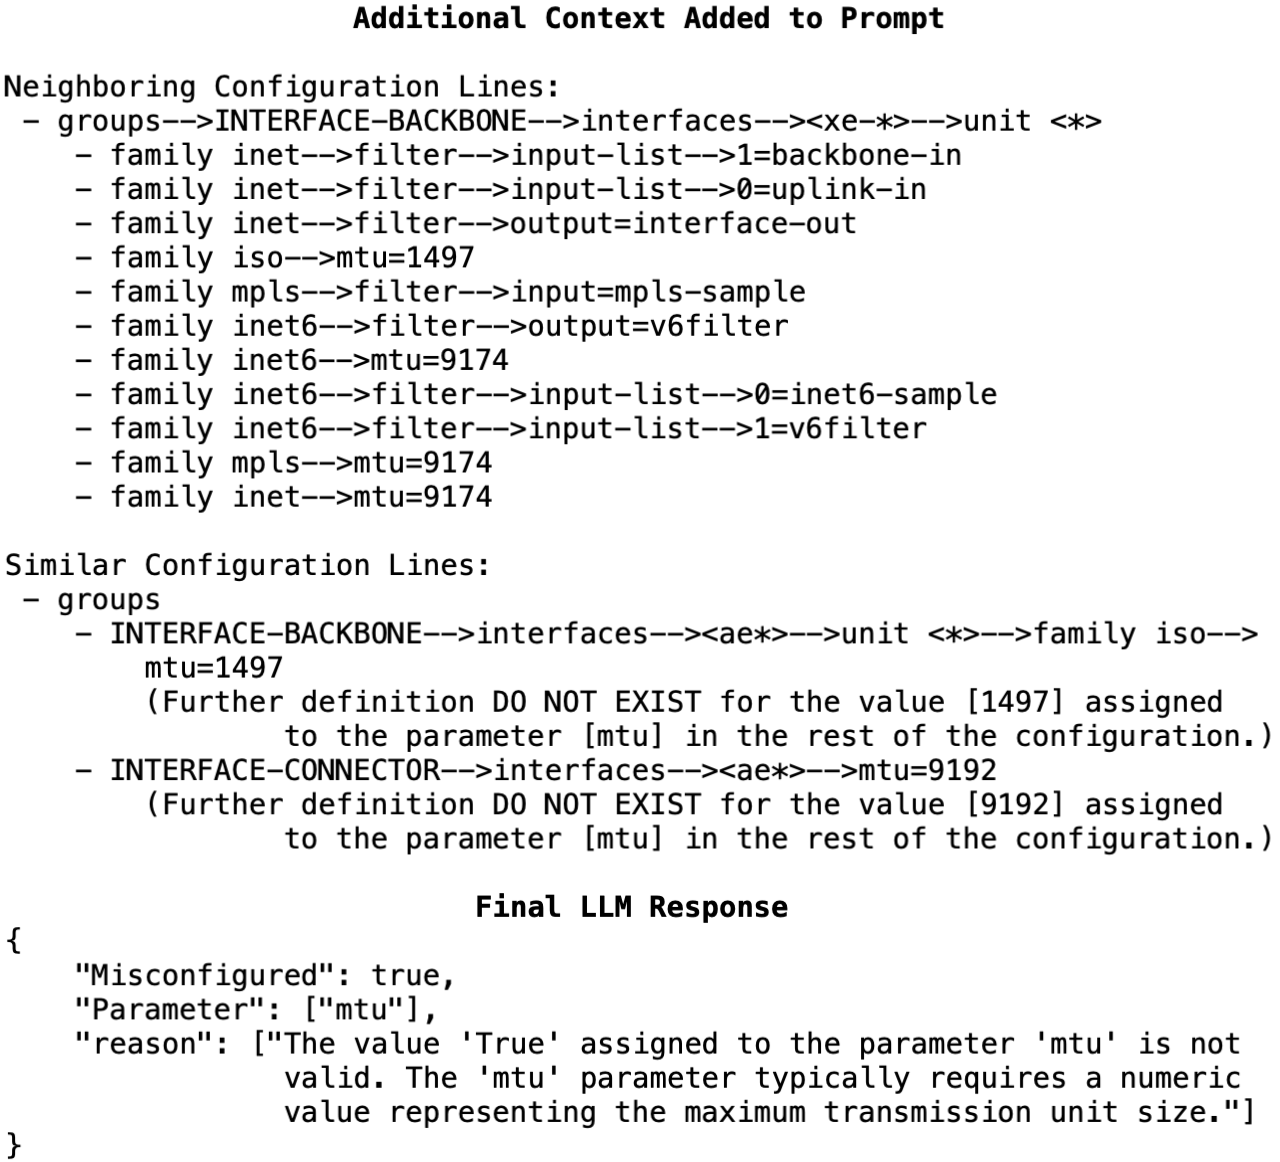
\includegraphics[width=0.95\columnwidth]{figs/feedback_and_response.png}}
    \caption{Example: Adding requested context and retrieving misconfiguration detection result.}
    \label{fig:feedback_and_response}
\end{figure}


This sequential, interactive approach mirrors how a network administrator might manually review a configuration file—examining the most relevant sections first, then digging deeper into referenceable or adjacent configurations as needed.

% It ensures that the model focuses on the most critical aspects of the configuration without becoming overwhelmed by extraneous information.

\mypara{Why Iterative, Requested Based Prompting Works:}
By breaking down the context into smaller, more digestible portions, \sysname{} addresses the fundamental challenges of context overload. This method significantly enhances the model’s ability to:
\begin{enumerate}
    \item Stay on target: With less irrelevant information, the model can maintain focus on the specific issue under review.
    \item Preserve coherence: Incrementally adding information allows the model to build a more coherent understanding of the configuration~\cite{li2023prompt,subramonyam2024bridging}, improving detection of complex issues such as dependency conflicts or misapplied policies.
    \item Optimize performance: Avoiding context overload reduces the processing burden on the model, leading to faster and more reliable outputs.
\end{enumerate}

For example, in detecting misconfigurations in a multi-layer firewall policy, \sysname{} might first present the core rule in question, then iteratively offer neighboring rules that affect the same traffic flow, followed by referenceable configuration sections that define broader network policies. This structured process ensures that the LLM has all the information it needs, without drowning in unnecessary details, enabling it to make accurate decisions. Unlike conventional prompt-chaining, which provides incremental instructions based on a fixed context, \sysname{} dynamically adds context as requested by the LLM, focusing on the evolving needs of the analysis.

% By combining efficient context extraction with iterative, focused interaction, \sysname{} represents a significant advancement in leveraging LLMs for router misconfiguration detection, ensuring that models are both effective and computationally efficient.
